

In the rest of this thesis, we present our approaches that contribute to achieve our goal of code generators testing and compilers auto-tuning. Figure \ref{fig:overview} depicts an overview of how the different contributions we propose are connected to each other and how they contribute to achieve the common goal.`

\begin{figure}[h]
	\center
	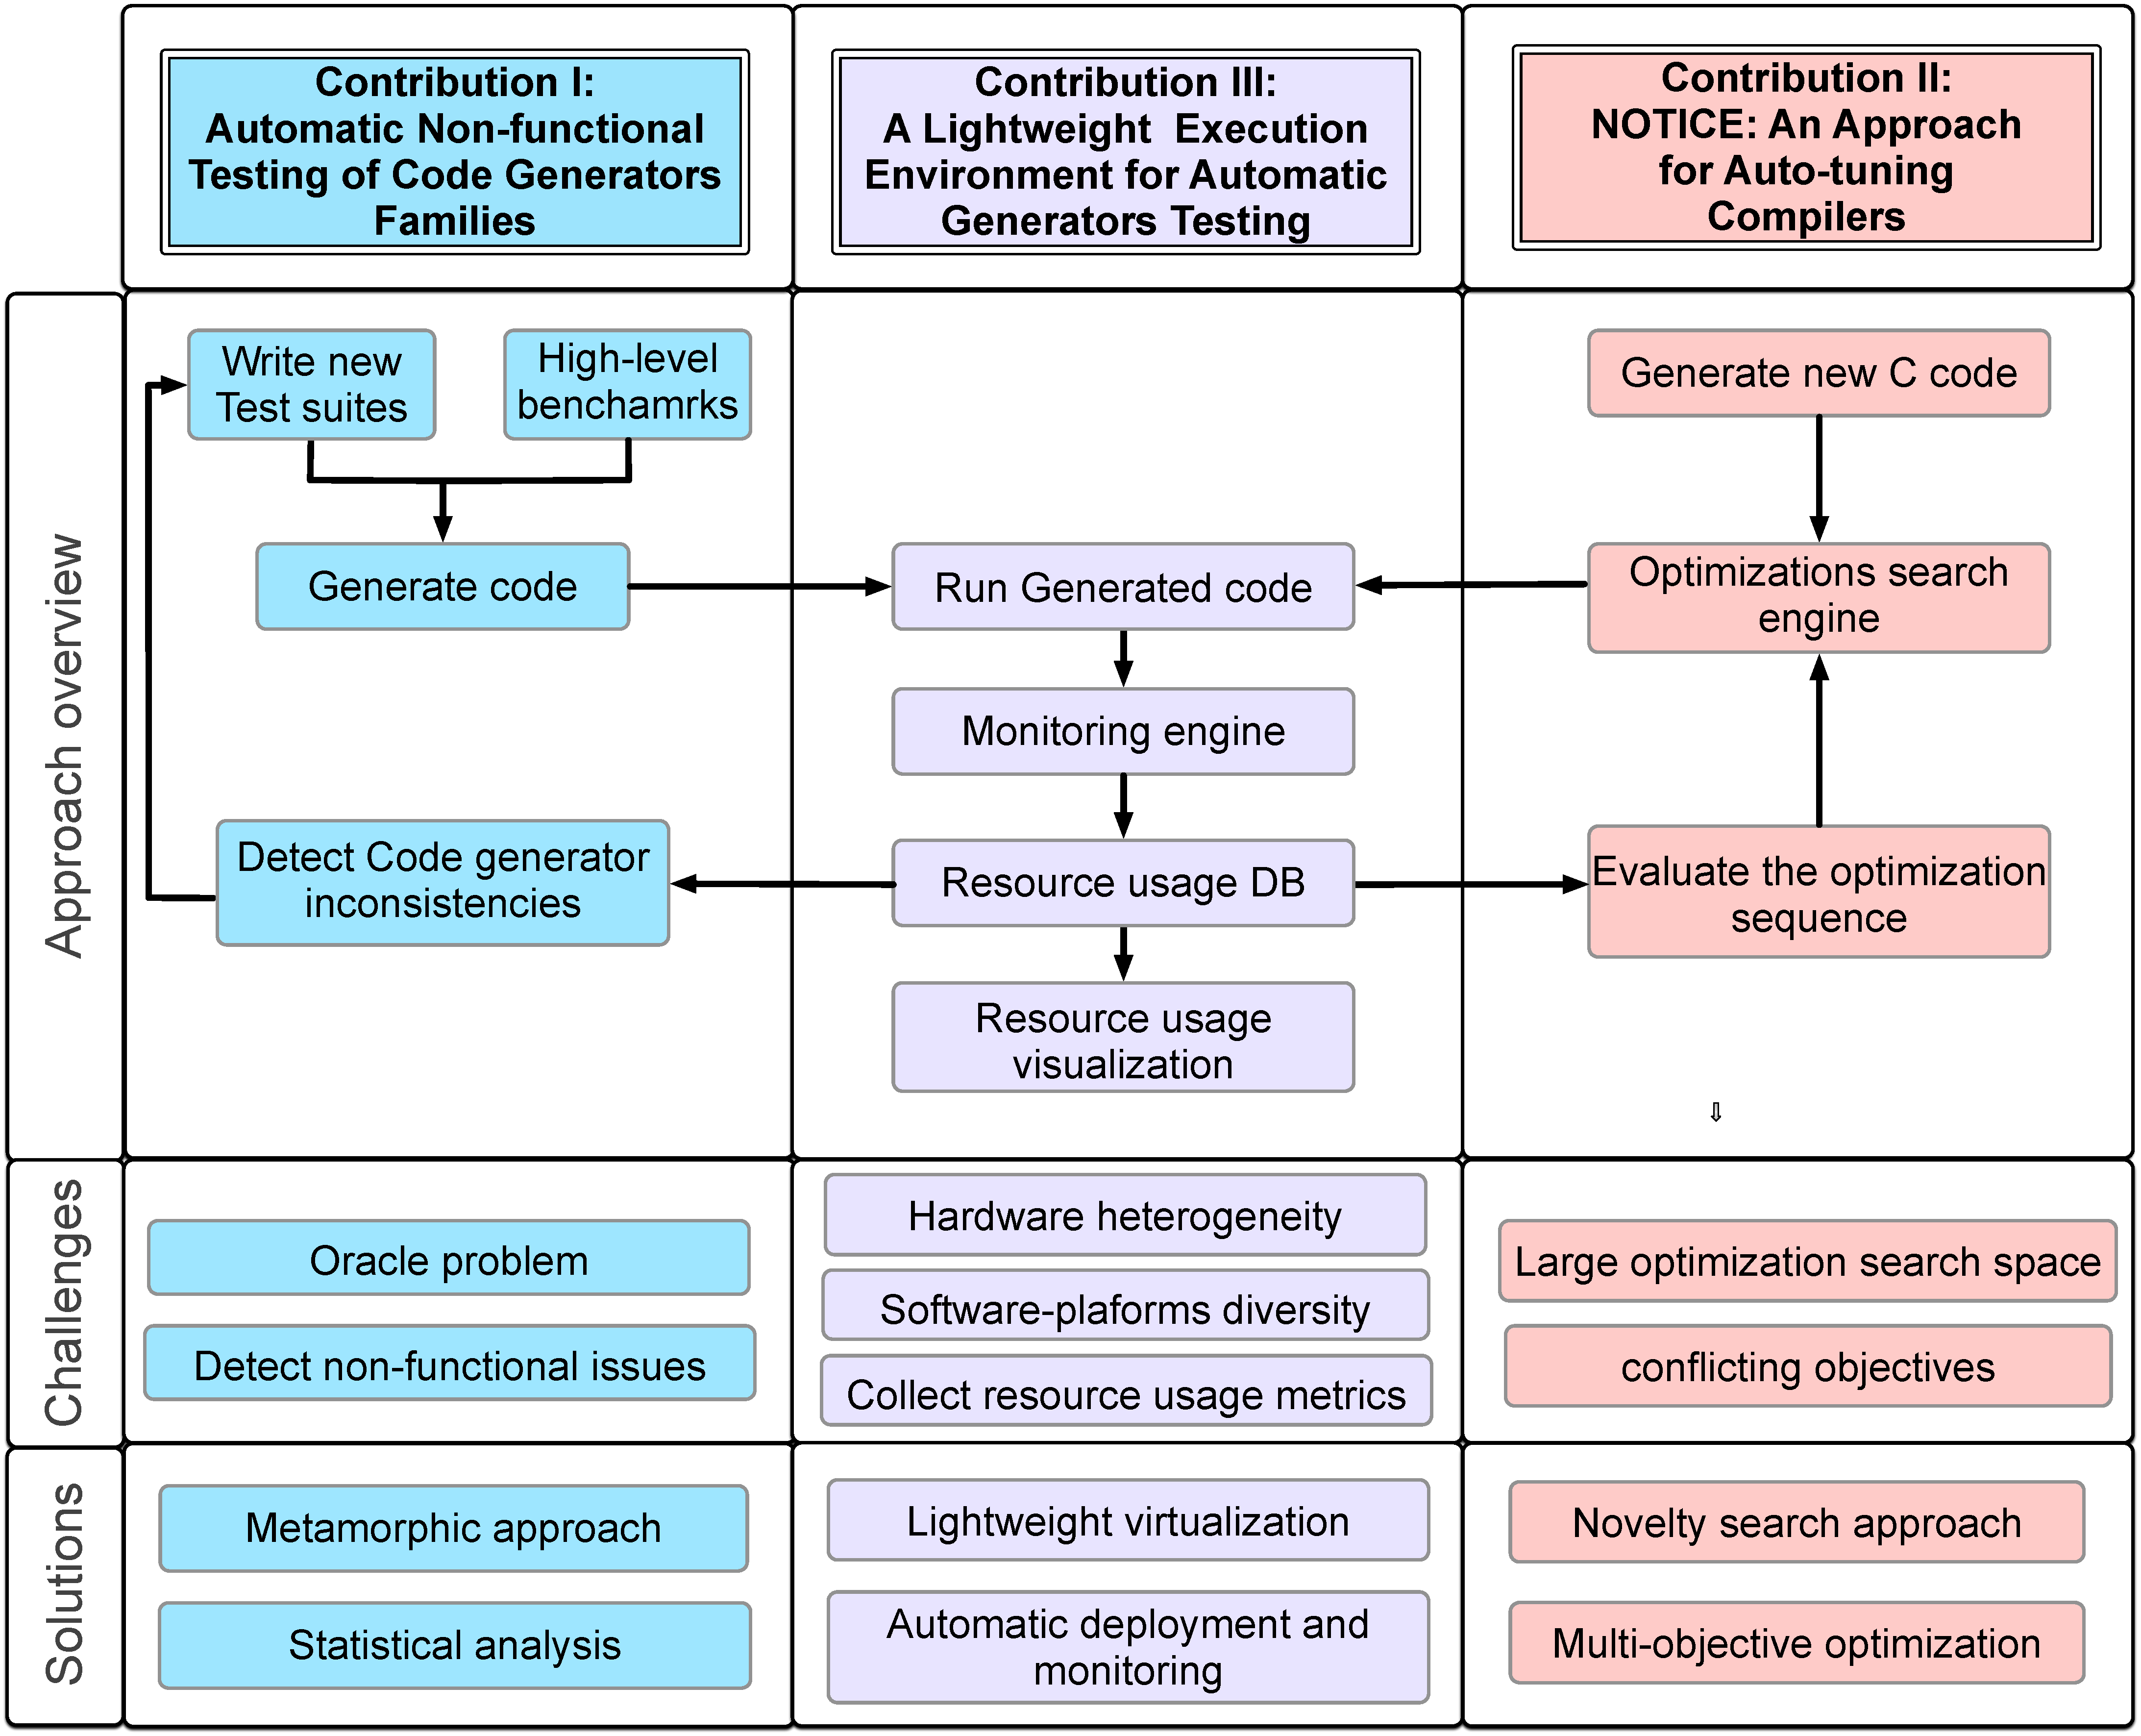
\includegraphics[scale=0.23]{Chapitre0/fig/overview}
	\caption{Summary of contributions}
	\label{fig:overview}
\end{figure}

This thesis makes three contributions:
\begin{itemize}
	\item \textbf{Code generators testing (in red): }
	
	In this contribution (chapter 4), we propose an approach for testing code generators. To do so, we create high-level benchmarks and test suites using Haxe. Afterwards, we generate automatically source code to five different target languages (Java, C++, C\#, PHP and JS). Code execution and runtime monitoring is ensured by the third contribution relative to the code execution and monitoring in a sandbox environment. In this contribution, we rather focus  on presenting an automatic way for detecting inconsistencies within code generator families.
	
	\item \textbf{Compilers auto-testing (in green):}
	
	As discussed in the state of the art, compilers auto-testing is part of the iterative compilation research field. Thus, we present in chapter 5, an adaptation of the novelty search algorithm for compilers auto-tuning. Our contribution focuses on tuning GCC compilers based on randomly generated C programs.
	This approach shares the same monitoring infrastructure as the previous contribution in order to evaluate the impact of discovered optimization sequences on resource usage. The outcome of this approach is the best set of optimizations sequences for a giving hardware architecture, a given input program and for a specific resource usage metric. 
	
	\item \textbf{Resource usage monitoring infrastructure (in yellow):}
	
	We propose in chapter 6, an infrastructure based on micro-services namely Docker in order to automate the software deployment, execution and monitoring. It provides for the first contribution information about the resource usage of generated programs. For the second contribution, it provides as well information about the quality of optimized code in terms of memory and CPU usage. Finally, we provide also in this contribution a mechanism to visualize at runtime the resource usage of running programs.
\end{itemize}

The validation of each contribution is presented in the corresponding chapter. Different experiments are used to illustrate the characteristics of each solution we present.



